\documentclass[letterpaper, 12pt]{article}
\usepackage[top=.5in,bottom=.5in,left=.75in,right=.75in,headheight=30pt, % as per the warning by fancyhdr
includehead,includefoot,
heightrounded, % to avoid spurious underfull messages
]{geometry}
\addtolength{\topmargin}{-.25in}
\usepackage{fancyhdr}
\pagestyle{fancy}
\usepackage{graphicx}
\usepackage{lastpage}
\usepackage{multicol}
\newcommand{\assnum}{Assignment 8.01}
\newcommand{\assname}{Centripetal Force and Acceleration KEY}
\usepackage{xcolor}
\usepackage[makeroom]{cancel}

\begin{document}
\fancyhead[l]{	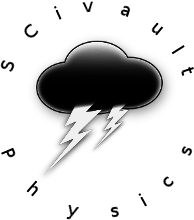
\includegraphics[height=0.5in]{../Logo/sp.png} Name:  \color{red} KEY - DO NOT REPRODUCE \color{black} }
\fancyhead[r]{Due Date: \hspace{ 1in}}
\fancyfoot[c]{\thepage\ of \pageref{LastPage}}
\fancyfoot[r]{\assnum}	


\begin{center} \assnum{} - \assname{}
\end{center}

\begin{enumerate}
	\item A carnival ride has a circular wheel with a radius of 3 meters.  It rotates with a tangential velocity of 10 m/s.  What is the acceleration that a person on this ride will feel?
		
		\color{red}
		\begin{center}
		$ a_c = \frac{v^2}{r} = \frac{(10m/s)^2}{3m} = 33.333 m/s^2
		\vspace{.15in} 			$
		\end{center}
		\color{black}
	
	\item You are swinging a bucket of water around in a vertical circle, with a radius of 1 meter.  
	\begin{enumerate}
		\item What is the minimum velocity you must swing the bucket with in order to keep the water in the bucket?
		\vspace{.25in} 	
		\color{red}
		\begin{center}
		$ a_c = \frac{v^2}{r} \Longrightarrow v = \sqrt{a_cr} = \sqrt{(9.81m/s^2)(1m)} \approx 3.132 m/s
		\vspace{.25in} 			$
		\end{center}
		\color{black}
	
	
	
		\item 	How long would it take to make one full rotation?
			\vspace{.25in} 	
			
		\color{red}
		\begin{center}
			$ v = \frac{d}{t} \Longrightarrow t = \frac{d}{v} =  \frac{c}{v} = \frac {2 \pi r} {v} = \frac {2 \cdot \pi \cdot 1 m} {3.132 m/s} \approx 2.006 s		$
		\end{center}
		\color{black}
		
		
		
		
		
		
	\end{enumerate}
	
	\item A compact disk will shatter if its rotational rate exceeds 28,000 rotations per minute.  A CD has a radius of 0.08 meters.
		\begin{enumerate}
			\item Calculate the speed at which the CD will shatter.
				\vspace{1in}
			\item A section of CD, at a distance of 7 cm from the center of the disk has a mass of 1.2 grams. What is the force on this section of the CD?
				\vspace{1in}
		\end{enumerate}
	
	\item In a move, Batman holds on to a helicopter rotor as it spins, before climbing into the helicopter. The helicopter has blades that are 4 meters long, and rotate 3 times per second.  
	\begin{enumerate}
		\item What is the circumference of the circle made by the helicopter blades?   
			\vspace{0.75in}
		\item 	What is the velocity that the blades rotate with?		
			\vspace{0.75in}
		\item What is the acceleration that batman feels?  How many g's is this?
			\vspace{0.75in}
		\item If batman has a mass of 80 kg, what is the force that he feels?
			\vspace{0.75in}
		\item What happens to Batman?	
			\vspace{0.75in}
	\end{enumerate}
	
	\item A penny is placed on top of a horizontal turntable, 5 cm from the axis of rotation.  The coefficient of friction between the turntable and the penny is 0.25.  If the mass of the penny is 0.0025 kg, at what speed would the turntable cause the penny to slide off?
	



\end{enumerate}
 



\end{document}
